\subsection{Tree Traversal}
\label{sec:traversal}
% At each step you reason about tradeoffs/alternative design choices and
% justify why you did it in the way you did it (advantages/shortcommings,
% and why your approach is reasonable). Of course mostly related to performance.

% Whenever possible, support your reasoning with (as in point to) experimental
% evaluation results (next).

\begin{itemize}
	\item using an integer to represent the stack
	\item the first traversal logic (show figure)
	\item the continuous traversal logic (show figure)
	\item checking a median on one dimension
	\item checking all medians from all dimensions (show equation)
	\item 
	\item 
	\item 
\end{itemize}	


As mention in the Background, Futhark does not support recursion, which is why the pseudo-code from Algorithm 3 is rewritten into an imperative version. One such solution is using a stack to traverse the tree incrementally while deciding which nodes to visit next. The figure below demonstrates the traverse down to the first leaf; this example does not need a stack because, at this point, we do not know if we need to visit additional leaves. Figures X-X show the traversal continuing from the first leaf, in which a stack is necessary. 


\subsubsection{Representing the Stack as an Integer}

The naive solution of representing a stack is using a boolean list where the leaves and node are set to true once visited. Although this is a simple and correct solution, since the height of the tree never exceeds 32, it can be further optimised as an integer representation instead. The code in listing XX shows the bit arithmetic done to modify the right areas of the stack and the logic behind setVisited is demonstrated in XX. 

\begin{listing}[H]
\begin{minted}{haskell}
  let setVisited (stk: i32) (c: i32) : i32 =
      stk | (1 << c)
  let resetVisit (stk: i32) (c: i32) : i32 =
      stk & !(1 << c)
  let isVisited (stk: i32) (c: i32) : bool =
      (stk & (1 << c)) > 0i32
\end{minted}
\caption{Snippet of bit arithmetic for stack modifications.}
\label{lst:stack}
\end{listing}

\begin{figure}\label{fig:bits}
\begin{align*}
	&& &00000000000000000000100010000101 &\\ \text{or} 
	&& &00000000000000000000001000000000 &\\ 
	\cline{3-4}
	&& &00000000000000000000101010000101
\end{align*}
\caption{Example of stack integer arithmetic.}
\end{figure}



% \begin{align*}
% 	&& &00000000000000000000101010000101 &\\ \text{and} 
% 	&& &11111111111111111111110111111111 &\\ 
% 	\cline{3-4}
% 	&& &00000000000000000000100010000101
% \end{align*}





% \begin{listing}[H]
% \begin{minted}{haskell}
% entry firstTraverse [d][q] (height:   i32)  (median_dims: [q]i32)
%                            (query: [d]f32)  (median_vals: [q]f32) =

%     let new_leaf = loop node_index = 0
%         while !(isLeaf height node_index) do
%           if query[median_dims[node_index]] <= median_vals[node_index]
%           then (node_index+1)*2-1
%           else (node_index+1)*2

%     in new_leaf
% \end{minted}
% \caption{Futhark implementation of the first tree traversal.}
% \label{lst:first}
% \end{listing}



% \begin{figure}[H]
% \centering
% 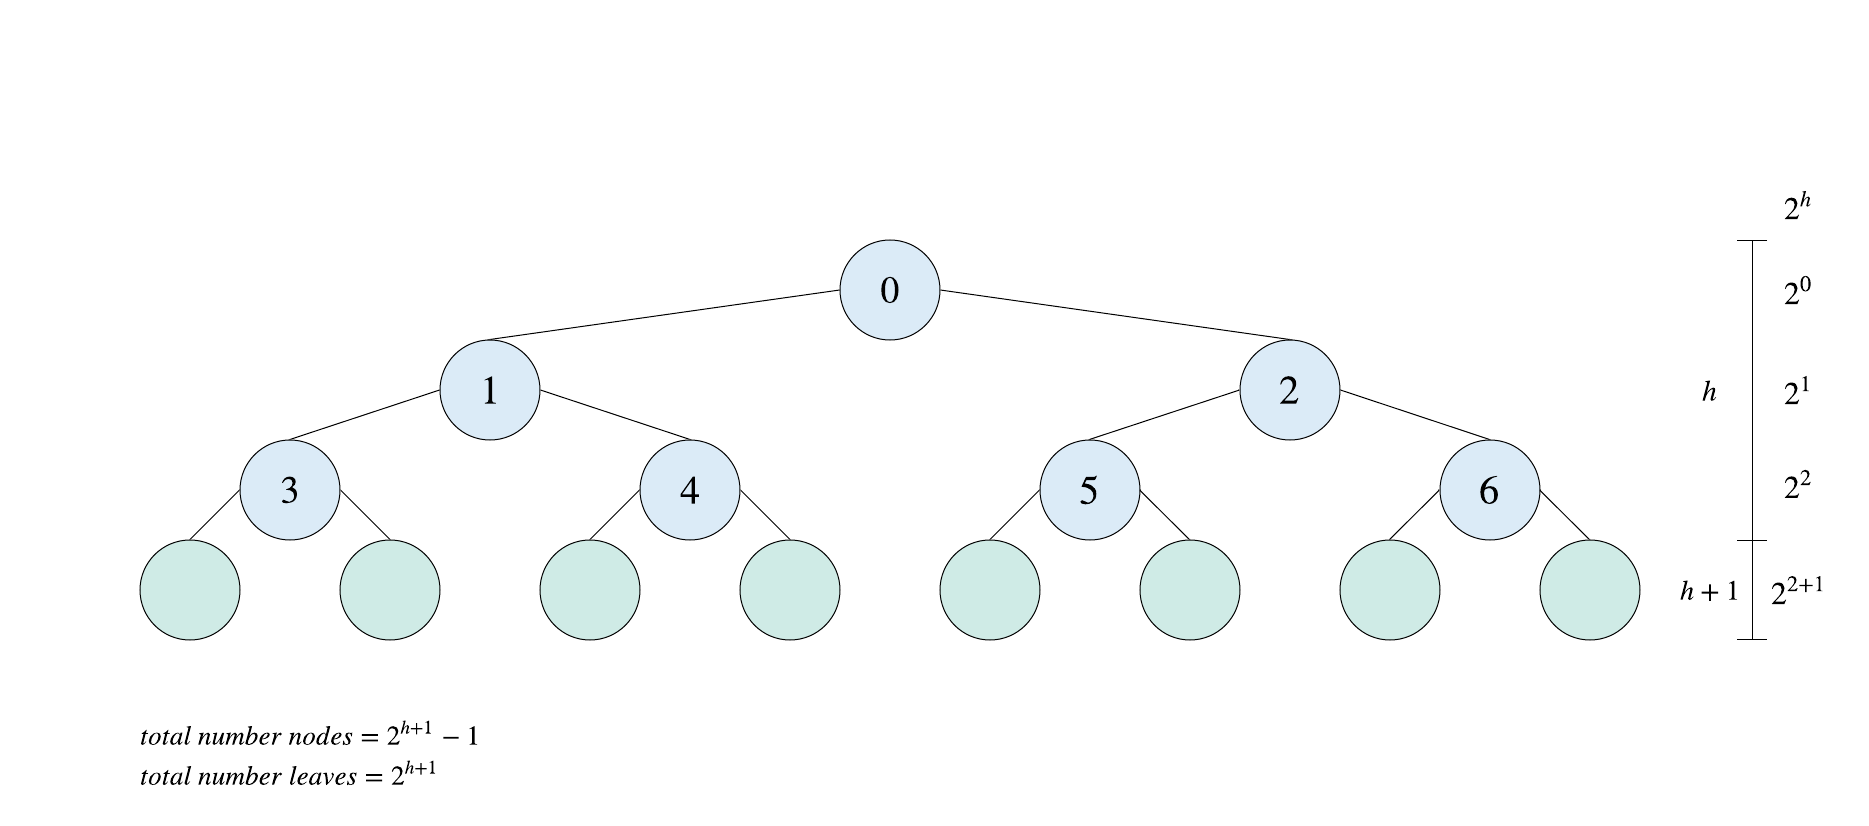
\includegraphics[width=0.9\textwidth]{pics/kd-tree-visual/1.png}
% \caption{}
% \end{figure}


\begin{figure}[H]
\centering
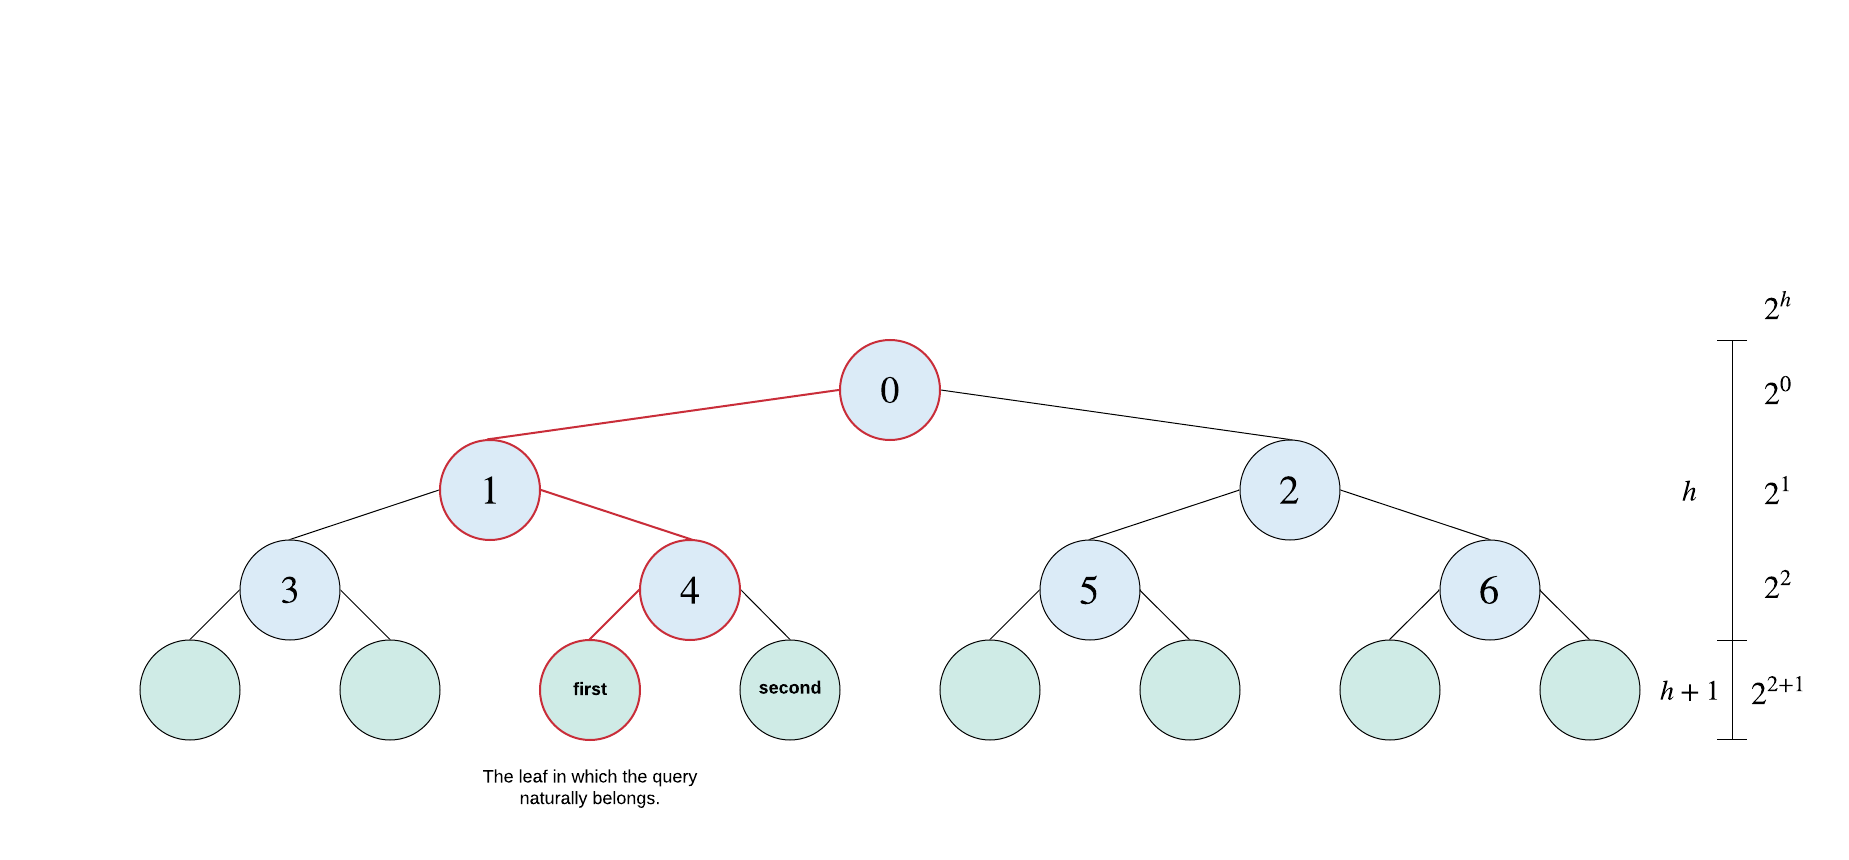
\includegraphics[width=0.9\textwidth]{pics/kd-tree-visual/22.png}
\caption{}
\end{figure}

\begin{figure}[H]
\centering
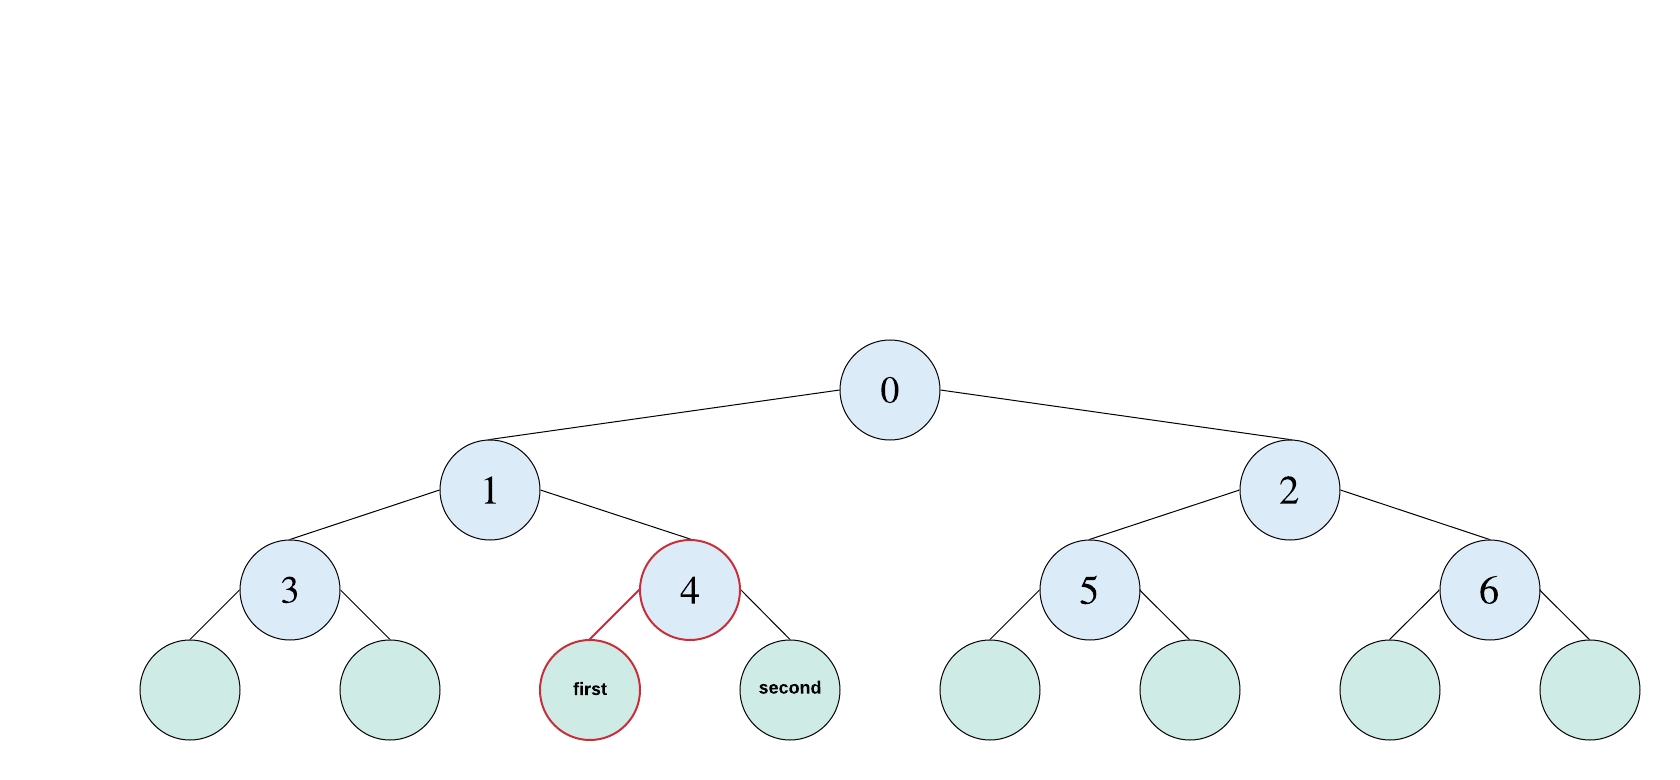
\includegraphics[width=0.9\textwidth]{pics/kd-tree-visual/3.png}
\caption{}
\end{figure}

% \begin{figure}[H]
% \centering
% 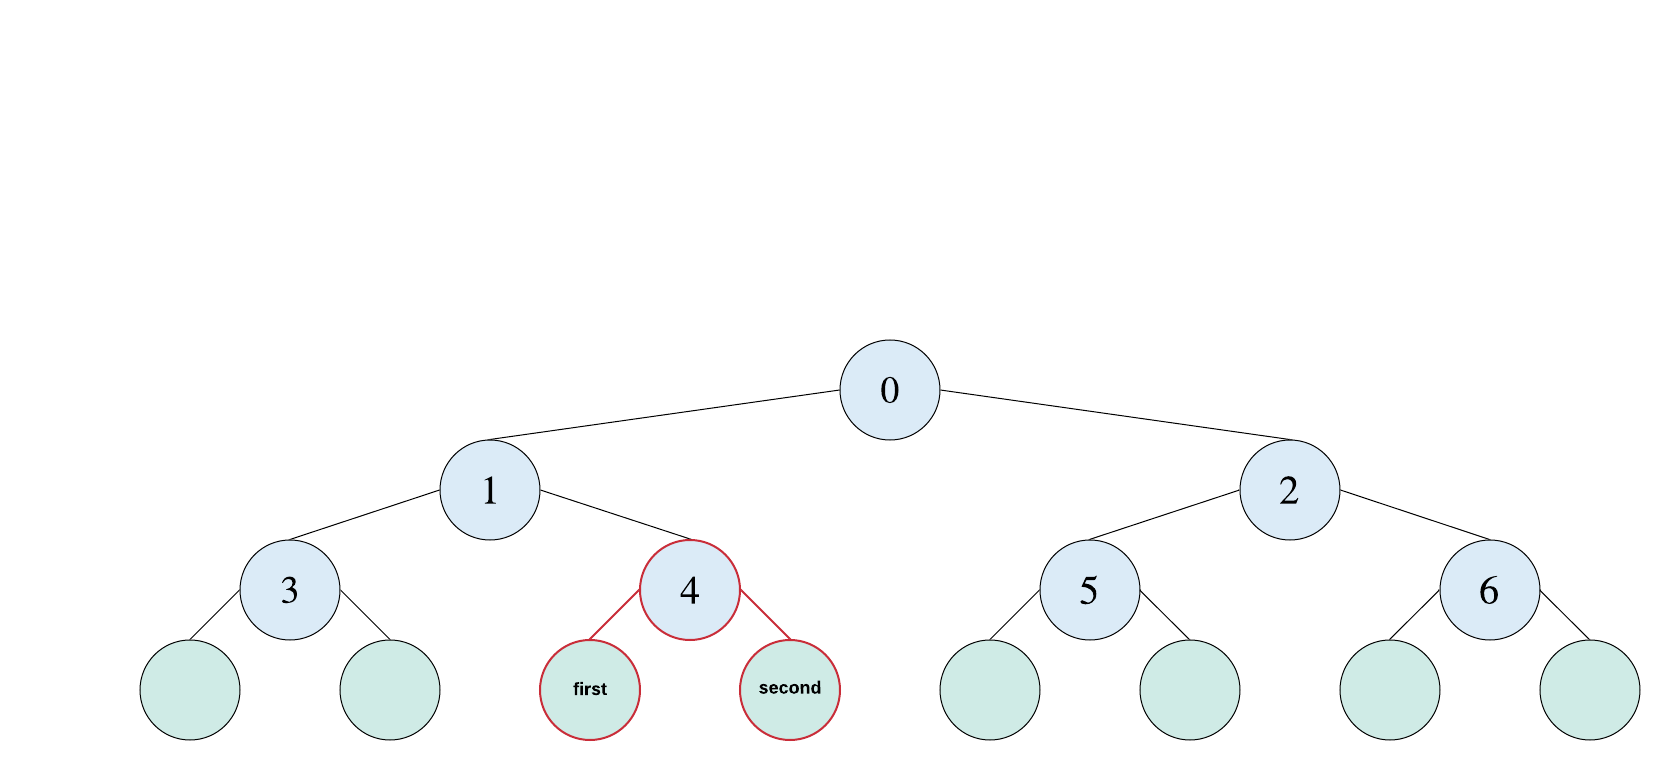
\includegraphics[width=0.9\textwidth]{pics/kd-tree-visual/4.png}
% \caption{}
% \end{figure}

\begin{figure}[H]
\centering
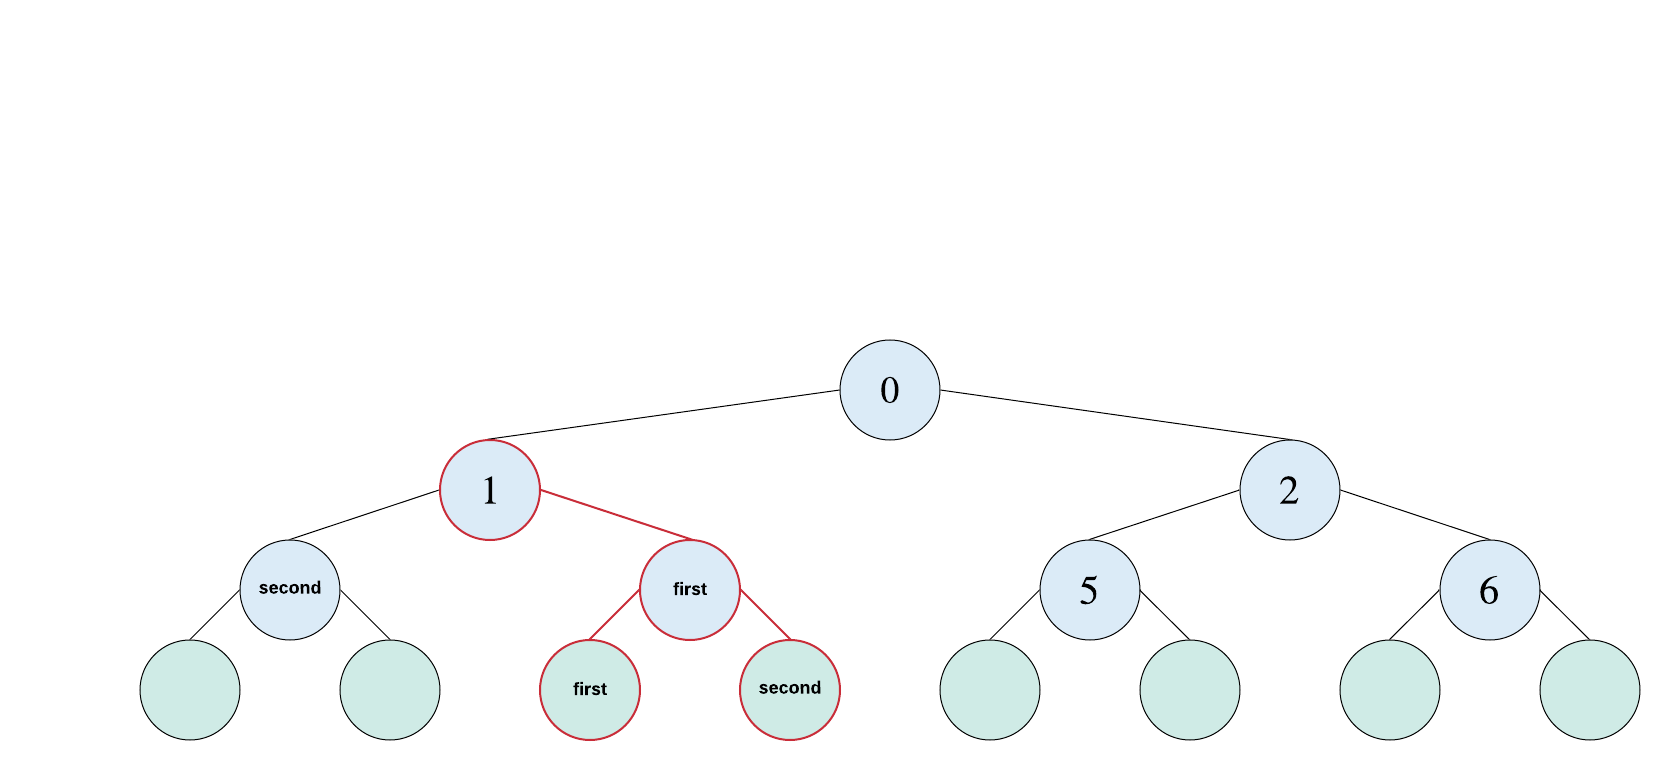
\includegraphics[width=0.9\textwidth]{pics/kd-tree-visual/5.png}
\caption{}
\end{figure}

% \begin{figure}[H]
% \centering
% 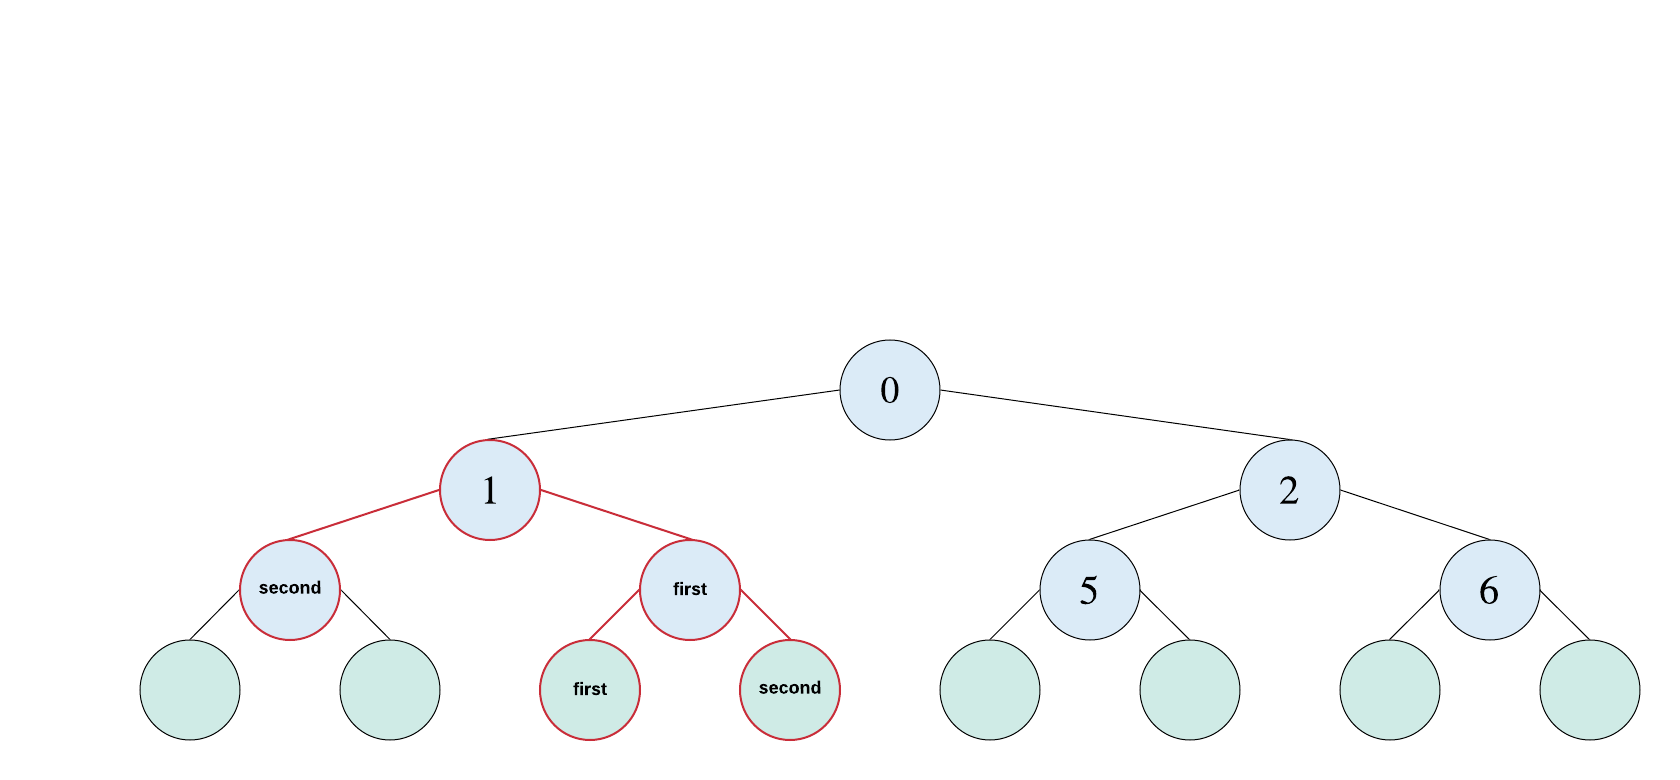
\includegraphics[width=0.9\textwidth]{pics/kd-tree-visual/6.png}
% \caption{}
% \end{figure}

\begin{figure}[H]
\centering
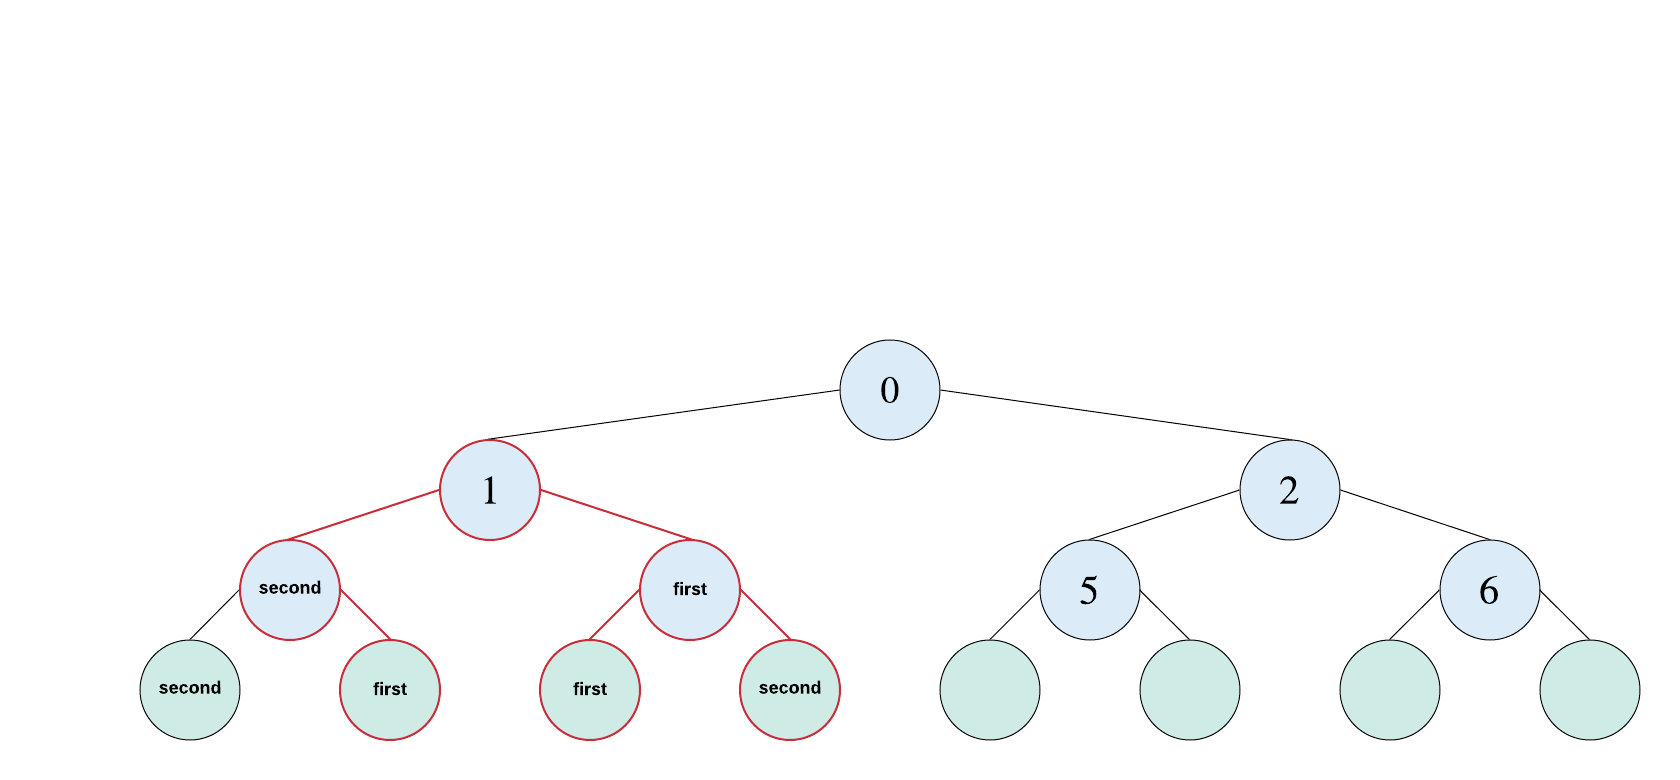
\includegraphics[width=0.9\textwidth]{pics/kd-tree-visual/7.png}
\caption{}
\end{figure}

% \begin{figure}[H]
% \centering
% 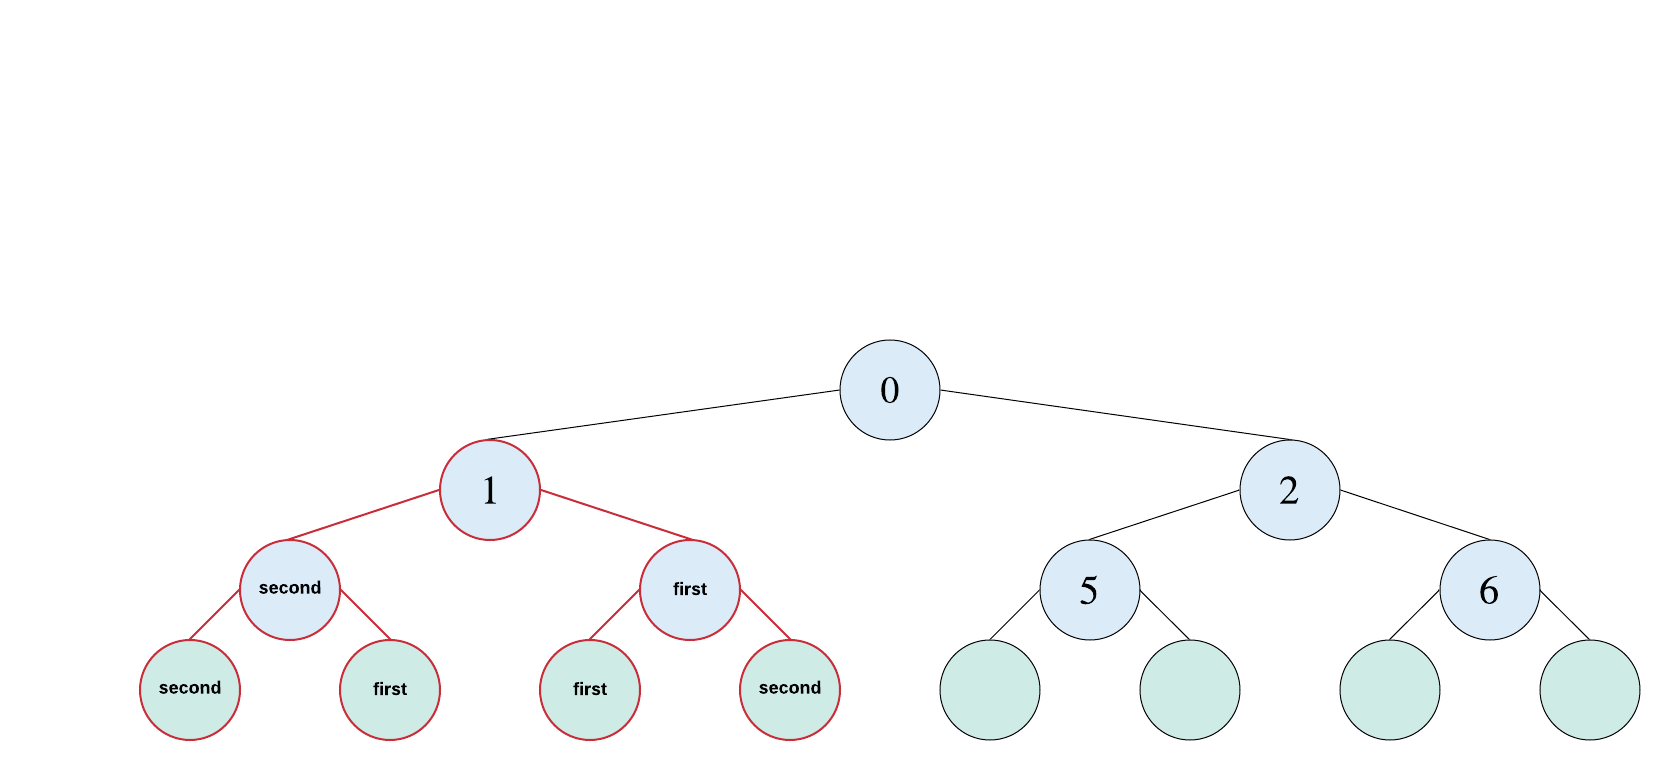
\includegraphics[width=0.9\textwidth]{pics/kd-tree-visual/8.png}
% \caption{}
% \end{figure}

% \begin{figure}[H]
% \centering
% 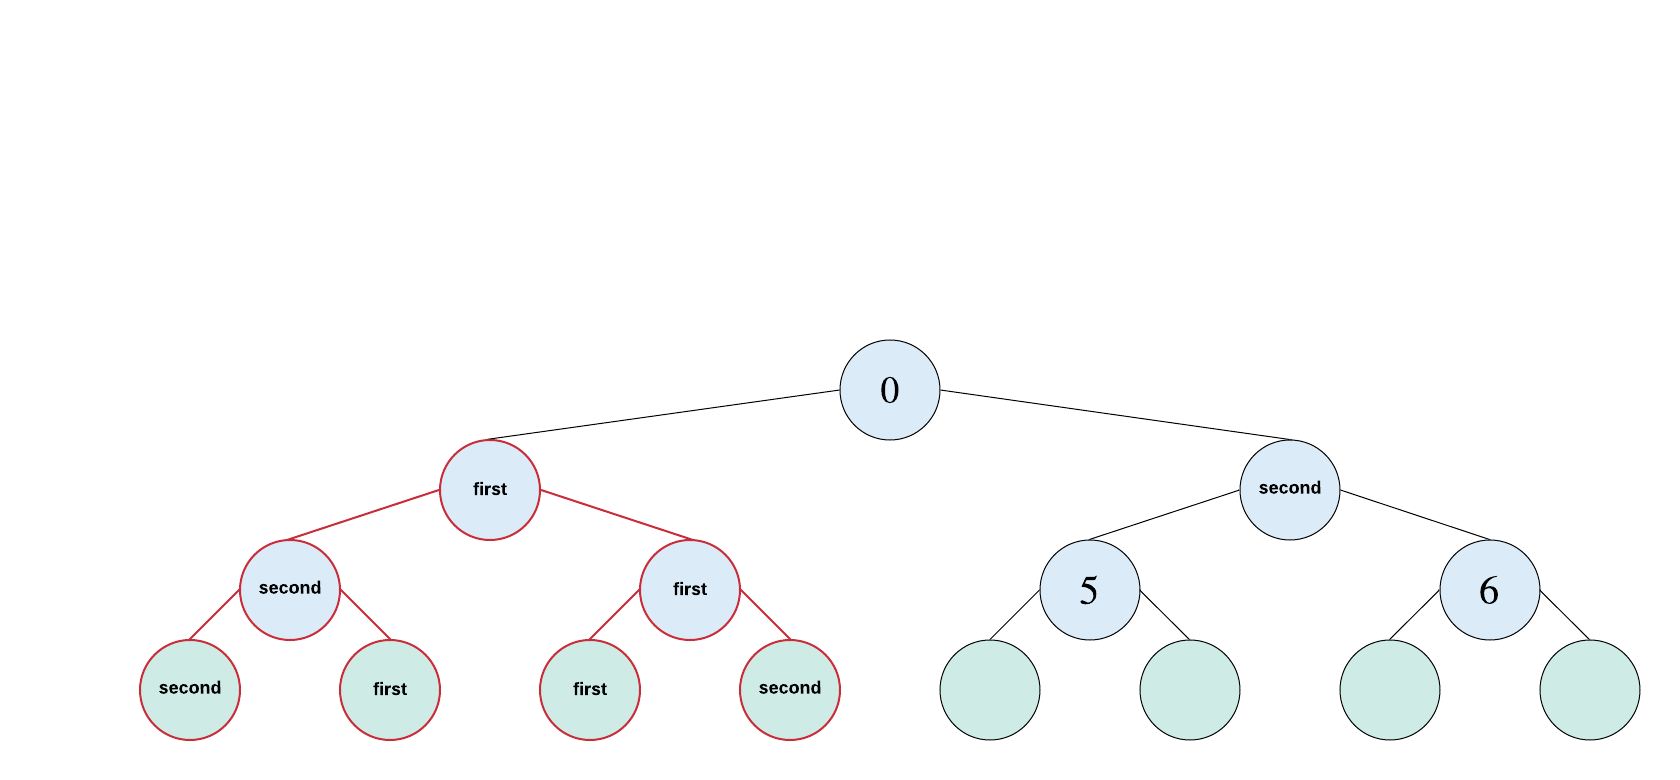
\includegraphics[width=0.9\textwidth]{pics/kd-tree-visual/9.png}
% \caption{}
% \end{figure}

\begin{figure}[H]
\centering
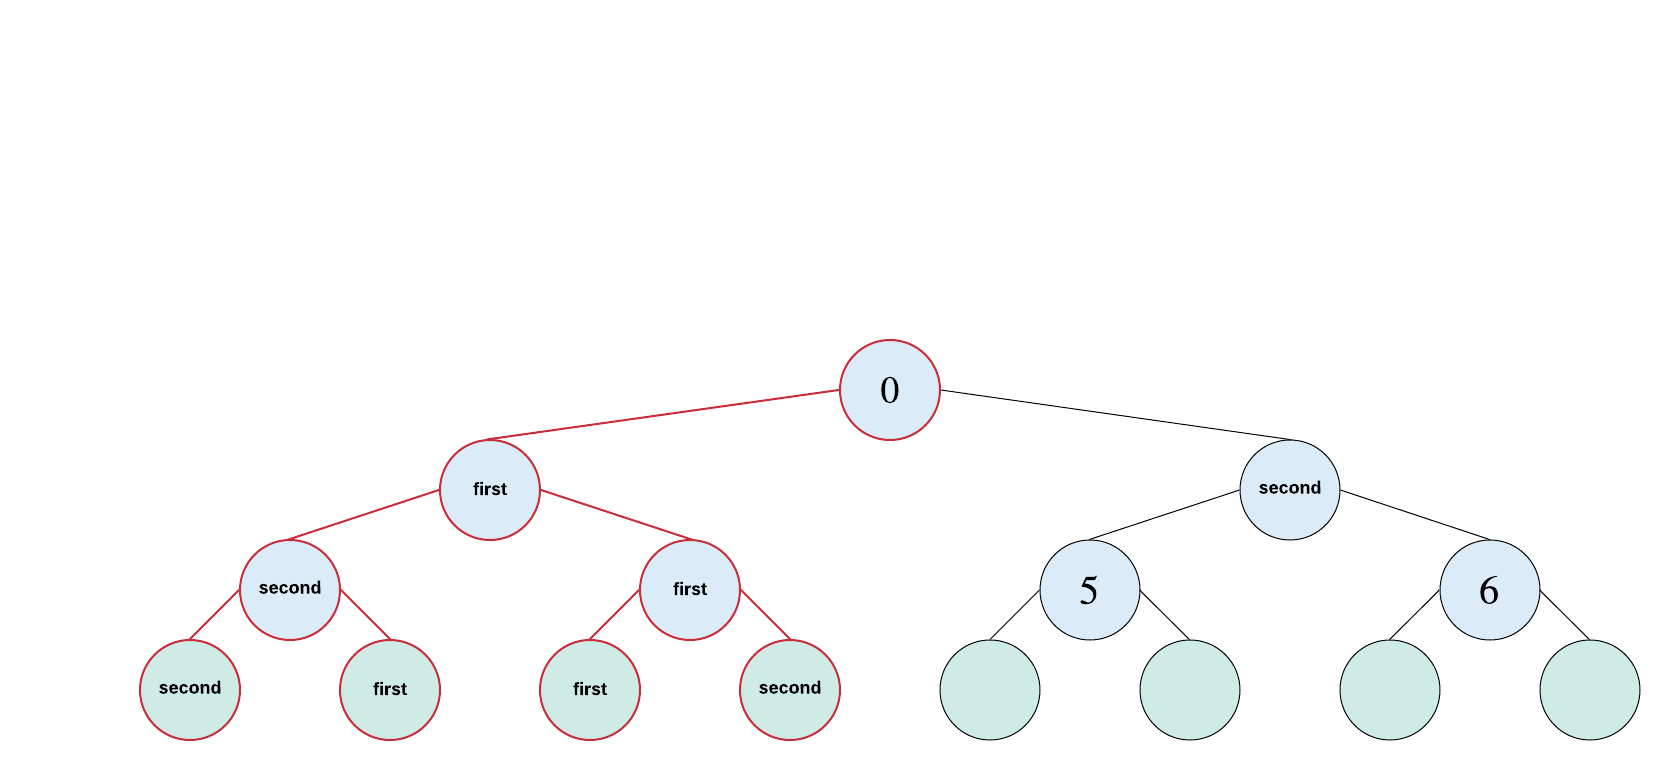
\includegraphics[width=0.9\textwidth]{pics/kd-tree-visual/10.png}
\caption{}
\end{figure}

\begin{figure}[H]
\centering
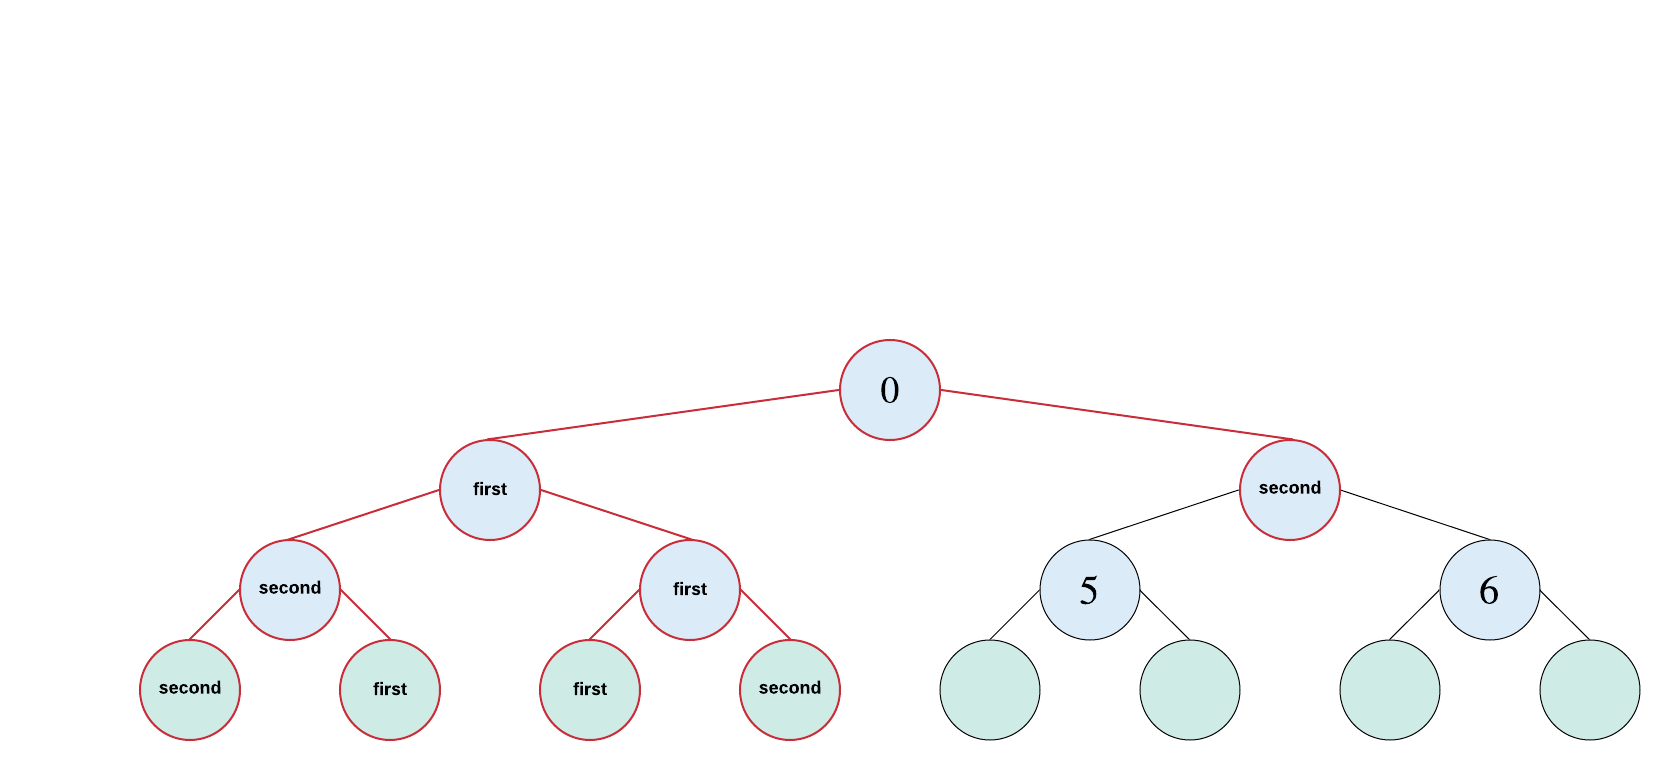
\includegraphics[width=0.9\textwidth]{pics/kd-tree-visual/11.png}
\caption{}
\end{figure}




\subsubsection{Validating Whether to Look at the \texttt{second}}

The original solution determines whether to visit the second node by XXX. 










\begin{listing}[H]
\begin{minted}{haskell}
entry traverse [d][n][l] (height:             i32)  (median_dims:     [n]i32)
                         (median_vals:     [n]f32)  (wknn:               f32)
                         (query:           [d]f32)  (stack:              i32) 
                         (last_leaf:          i32)  (lower_bounds: [l][d]f32)
                         (upper_bounds: [l][d]f32)  : (i32, i32) =

  let setVisited (stk: i32) (c: i32) : i32 =
      stk | (1 << c)
  let resetVisit (stk: i32) (c: i32) : i32 =
      stk & !(1 << c)
  let isVisited (stk: i32) (c: i32) : bool =
      (stk & (1 << c)) > 0i32

  let (parent_rec, stack, count, rec_node) =
      loop (node_index, stack, count, rec_node) =
           (last_leaf, stack, height, -1)
            while (node_index != 0) && (rec_node < 0) do
                let parent = getParent node_index
                let second = node_index + addToSecond node_index in

                if isVisited stack count
                then (parent, stack, count-1, -1)
                else
                  let ack = 
                    loop ack = 0.0f32
                      for i < d do
                          let cur_q = query[i]
                          let lower = lower_bounds[second,i]
                          let upper = upper_bounds[second,i] in

                          if cur_q <= lower then
                              let res = (cur_q-lower)*(cur_q-lower)
                              in (ack + res)
                          else if cur_q >= upper then
                              let res = (cur_q-upper)*(cur_q-upper)
                              in (ack + res)
                          else (ack + 0.0)

                  let to_visit = (f32.sqrt ack) < wknn in
                  let to_visit = f32.abs(median_vals[parent] - query[median_dims[parent]]) < wknn in
                  if !to_visit
                  then (parent, stack, count-1, -1)
                  else
                    let second = node_index + addToSecond node_index
                    let stack  = setVisited stack count in
                    (parent, stack, count, second)


  let (new_leaf, stack, _) =
      if parent_rec == 0 && rec_node == -1
      then (-1, stack, 0)

      else loop (node_index, stack, count) =
                (rec_node, stack, count)
           while !(isLeaf height node_index) do
              let count = count + 1
              let stack = resetVisit stack count in
              if query[median_dims[node_index]] <= median_vals[node_index]
              then ((node_index+1)*2-1, stack, count)
              else ((node_index+1)*2, stack, count)

  in (new_leaf, stack)
\end{minted}
\caption{Futhark implementation of the tree traversal.}
\label{lst:traverse}
\end{listing}
